\chapter{RESULTS}
\label{ch:results}

Evaluating the BioBERT triage classifier requires a structured analysis of predictive performance under domain shift and pathway implications. Architecture, TEWS, and the three training stages are specified in Chapter~\ref{ch:method} (Sections~\ref{sec:encoder},~\ref{sec:tews},~\ref{sec:training-pipeline}). Primary reported metrics come from \textbf{external} evaluation on the National Hospital Ambulatory Medical Care Survey (NHAMCS) 2018--22 and the Medical Information Mart for Intensive Care IV Emergency Department (MIMIC-IV-ED) open demo matching the v2.2 triage schema \citep{nhamcs201822,mimiciveddemo2023,mimicived2023}. Triagegeist is used for training and validation only. None of these sources is prospective live performance at \examplehospital{}, and the model has not yet been clinically tested on real patients there.

\section{Deployed checkpoints and evaluation setup}
\label{sec:biobert-analysis}

The deployed classifier is the Stage~3 fine-tuned model. Encoder architecture, TEWS, Stages~1--3, and Hugging Face identifiers are in Sections~\ref{sec:encoder},~\ref{sec:tews}, and~\ref{sec:training-pipeline} (Table~\ref{tab:model-ids}). External metrics follow in Section~\ref{sec:finetuned-analysis}.

Figure~\ref{fig:biobert-model-specs} shows the project inference configuration (\(M=128\)); see Section~\ref{sec:encoder} and \citet{lee2020biobert} for BioBERT-base constants.

\begin{figure}[H]
\centering
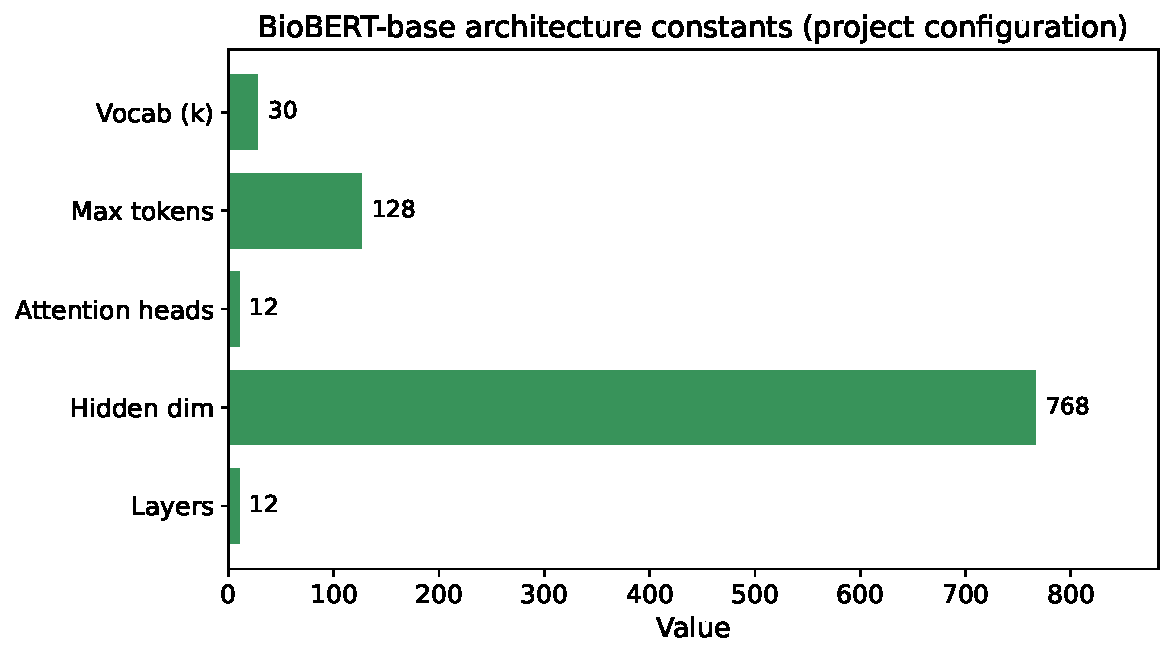
\includegraphics[width=0.88\textwidth]{figures/ch4/model_specs.pdf}
\caption{Project inference configuration constants (\(M=128\)); architecture in Section~\ref{sec:encoder}.}
\label{fig:biobert-model-specs}
\end{figure}

\section{Fine-tuned model analysis}
\label{sec:finetuned-analysis}

This chapter reports \textbf{external} predictive metrics, colour accuracy via \(f_{\mathrm{SATS}}\), under/over-triage, and pathway implications.

\subsection{Evaluation protocol}
\label{sec:eval-protocol}

Primary reported metrics are from external evaluation on MIMIC-IV-ED and NHAMCS. Triagegeist is used for training/validation only. The split was designed to reduce the risk of data leakage between Stage~3 training and published scores. None of these sources is prospective live performance at \examplehospital{}, and the model has not yet been clinically tested on real patients there.

\begin{enumerate}
\item \textbf{Train / validation (Triagegeist).} Stratified 90/10 split (seed~42) for Stage~3 fine-tuning and checkpoint selection. No Triagegeist holdout accuracy is reported as a Results headline.
\item \textbf{A: MIMIC-IV-ED.} Text-only on \texttt{chiefcomplaint} \(\rightarrow\) predict acuity; gold = \texttt{acuity} \(\in\{1,\ldots,5\}\). Full MIMIC-IV-ED v2.2 is credentialed on PhysioNet \citep{mimicived2023}; this project evaluates the open demo matching the same triage schema \citep{mimiciveddemo2023} (\(N=207\) after filters) until a full extract is available.
\item \textbf{B: NHAMCS 2018--22.} Text-only on \texttt{chief\_complaint\_text} \(\rightarrow\) predict acuity; gold = \texttt{target\_triage\_acuity} \citep{nhamcs201822}. After filters, \(N=58{,}124\) rows remain; metrics below use a stratified subsample of \(N=12{,}000\) (seed~42) for compute, with full-set class support reported in Table~\ref{tab:external-support}.
\end{enumerate}

\textbf{Pre-processing (both external sets).} Drop empty, NaN, or whitespace-only complaints; keep acuity in \(\{1,\ldots,5\}\); do \emph{not} expand nursing abbreviations (e.g.\ CP, SOB); tokenise with BioBERT WordPiece and truncate/pad to project length \(M=128\).

Two checkpoints are compared:

\begin{enumerate}
\item \textbf{Baseline fine-tuned BioBERT} (project default): end-to-end fine-tuning without minority rebalancing beyond the natural train distribution.
\item \textbf{Stratified-oversampling variant:} text augmentation plus random minority oversampling on the Triagegeist training split, then end-to-end fine-tuning (Section~\ref{sec:oversampling-choice}).
\end{enumerate}

Metrics: five-class accuracy and macro-F1; 4-colour accuracy after \(f_{\mathrm{SATS}}\); under-triage (predicted less urgent than true); over-triage (more urgent); critical under-triage (true Red\(\rightarrow\)non-Red; true Orange\(\rightarrow\)Yellow/Green); ordinal mean absolute error (MAE); latency.

\paragraph{Accuracy terminology.}
These quantities must not be blurred. \textbf{Five-class (text-classification) accuracy} is exact ESI-style level match. \textbf{Colour accuracy} is match after \(f_{\mathrm{SATS}}\) (Levels~4 and~5 both map to Green). \textbf{Gate accuracy} is clinical versus non-clinical discrimination on the contrast set (Section~\ref{sec:gate}), not acuity classification. \textbf{Clinical or pathway correctness} is not claimed from offline five-class or colour accuracy alone.

\paragraph{Error taxonomy.}
Classification, colour, and under-triage errors are related but not identical. For gold level \(y\) and prediction \(\hat{y}\),
\begin{align*}
  E_{\mathrm{class}} &= \mathbf{1}(\hat{y}\neq y), \\
  E_{\mathrm{colour}} &= \mathbf{1}\bigl(f_{\mathrm{SATS}}(\hat{y})\neq f_{\mathrm{SATS}}(y)\bigr), \\
  E_{\mathrm{under}} &= \mathbf{1}(\hat{y}> y)
\end{align*}
(with ESI convention that smaller integers are more urgent). Ordinal severity of class error is summarised by
\[
  \mathrm{MAE}=\frac{1}{N}\sum_{i=1}^{N}\lvert\hat{y}_i-y_i\rvert.
\]

\paragraph{Cost-sensitive objective (interpretive).}
Stakeholders may weigh under-triage, over-triage, and classification error differently. An interpretive risk functional (not used as the training loss in this project) is
\[
  R(\theta)=\lambda_u U(\theta)+\lambda_o O(\theta)+\lambda_e E(\theta),
\]
where \(U\) is under-triage rate, \(O\) is over-triage rate, \(E\) is five-class error rate, and \(\lambda_u,\lambda_o,\lambda_e\ge 0\) encode relative clinical cost. Stratified oversampling is interpreted as increasing emphasis on rare Red recall at the expense of \(E\) and often \(O\).

\subsection{Headline external metrics}
\label{sec:nhamcs-results}

Table~\ref{tab:external-metrics} is the primary results table for this chapter (NHAMCS and MIMIC demo; baseline vs stratified oversampling). Supporting acuity counts appear in Table~\ref{tab:external-support}.

\subsection{Acuity distribution on test sets}
\label{sec:external-support}

Table~\ref{tab:external-support} reports gold acuity counts by level after the shared pre-processing in Section~\ref{sec:eval-protocol}. The NHAMCS counts come from the 2018--22 US emergency-department survey text field \texttt{chief\_complaint\_text} with gold labels \texttt{target\_triage\_acuity} \citep{nhamcs201822}: \(N=58{,}124\) rows after filters, with the stratified evaluation subsample (\(N=12{,}000\)) used for published metrics. The MIMIC counts come from the open MIMIC-IV-ED demo on PhysioNet (Boston ED phrasing), mapping \texttt{chiefcomplaint} to gold \texttt{acuity} \citep{mimiciveddemo2023} (\(N=207\) after filters). Real emergency departments are imbalanced: NHAMCS is dominated by Levels~3--4, and Level~1 is scarce (846 of 58{,}124; 1.5\%). MIMIC demo counts are small, especially Levels~4--5, so rare-class metrics there are interpreted cautiously.

\begin{table}[H]
\centering
\small
\begin{tabular}{|l|r|r|r|r|r|r|}
\hline
\textbf{Set} & \(N_1\) & \(N_2\) & \(N_3\) & \(N_4\) & \(N_5\) & \textbf{Total} \\
\hline
NHAMCS (full retained) & 846 & 8{,}597 & 29{,}568 & 16{,}715 & 2{,}398 & 58{,}124 \\
NHAMCS (eval subsample) & 175 & 1{,}775 & 6{,}104 & 3{,}451 & 495 & 12{,}000 \\
MIMIC-IV-ED demo & 18 & 97 & 90 & 2 & 0 & 207 \\
\hline
\end{tabular}
\caption{Gold acuity counts by level on the NHAMCS and MIMIC-IV-ED demo test sets after pre-processing.}
\label{tab:external-support}
\end{table}

\subsection{Why prior in-distribution accuracy looked inflated}
\label{sec:high-accuracy}

Let \(N=80{,}000\) denote the Triagegeist training-pair count used for Stage~3. After normalising complaint strings, only
\[
  N_{\mathrm{unique}}=4{,}949
\]
distinct complaints remain, so the duplicate rate is
\[
  D=1-\frac{N_{\mathrm{unique}}}{N}=1-\frac{4{,}949}{80{,}000}\approx 0.9381
\]
(about 93.8\%; 4{,}184 templates appear at least five times). Random row-level splitting can therefore place near-identical linguistic templates in both training and validation folds, inflating in-distribution accuracy. High template reuse helps explain why earlier holdout figures near 99.9\% looked unrealistically strong: they largely measure agreement on repeated synthetic phrasing, not generalisation. Those figures are therefore retired from the Results headline in favour of MIMIC/NHAMCS metrics below. A full complaint-level deduplicated retrain is left as future work.

\subsection{Stratified oversampling for class imbalance}
\label{sec:oversampling-choice}

Stage~3 training on Triagegeist is class-imbalanced: Level~3 (Urgent) is the mode, while Level~1 (Resuscitation / Red) is the minority. Rebalancing the training split can raise Red recall, but often at a cost to precision and overall accuracy. Two natural ways to reduce that imbalance were available for this project.

\textbf{A: Classical embedding SMOTE.} Raw chief-complaint strings are discrete, so SMOTE cannot interpolate between token sequences directly \citep{chawla2002smote}. One workable route is to freeze (or otherwise detach) BioBERT, extract fixed feature vectors such as \(h_{[\mathrm{CLS}]}\in\mathbb{R}^{768}\), apply SMOTE in that continuous space to synthesise minority examples, and train a \emph{separate} linear classification head on the resulting embedding set. Gradients never update the text encoder during that second stage.

\textbf{B: Stratified oversampling (chosen).} Keep the end-to-end Stage~3 pipeline of Chapter~\ref{ch:method}: WordPiece tokenisation, BioBERT encoder, and Softmax head trained jointly. On the Triagegeist \emph{training} split only, apply text augmentation to minority urgent classes, then random minority oversampling toward configured target counts, and continue full encoder-plus-head updates. The training configuration sets \texttt{USE\_EMBEDDING\_SMOTE=False}, so embedding-space SMOTE is not part of the published second checkpoint.

This project adopts \textbf{B} for the published imbalance-mitigated checkpoint and does \emph{not} report a classical embedding-SMOTE model as the official second result.

The choice follows from the training objective. End-to-end Stage~3 is meant to adapt WordPiece and attention features to short chief-complaint language; that requires backpropagation into BioBERT. SMOTE-generated points in embedding space cannot be pushed back through the text encoder unless BioBERT is frozen, which would abandon that adaptation goal and replace it with a shallow head on static features. Stratified oversampling instead keeps real or lightly paraphrased complaint text inside the same tokenizer \(\rightarrow\) encoder \(\rightarrow\) Softmax path already specified in Chapter~\ref{ch:method}. Calling B ``SMOTE'' would therefore be inaccurate for the panel: Chawla-style SMOTE \citep{chawla2002smote} describes A, which was considered but not used for the published checkpoint.

The NHAMCS and MIMIC comparisons below therefore contrast the baseline Stage~3 model with this stratified-oversampling checkpoint, not with an embedding-SMOTE head.

\subsection{NHAMCS results}

Table~\ref{tab:external-metrics} summarises headline metrics on the stratified NHAMCS subsample (\(N=12{,}000\)) and, for comparison in the same panel, the MIMIC-IV-ED demo (\(N=207\)).

\begin{table}[H]
\centering
\small
\begin{tabular}{|l|r|r|r|r|}
\hline
\textbf{Metric} & \textbf{NHAMCS base.} & \textbf{NHAMCS overs.} & \textbf{MIMIC base.} & \textbf{MIMIC overs.} \\
\hline
\(N\) & 12{,}000 & 12{,}000 & 207 & 207 \\
Accuracy & 0.4760 & 0.3045 & 0.3043 & 0.2126 \\
Macro-F1 & 0.2882 & 0.2146 & 0.1748 & 0.1781 \\
Colour accuracy & 0.4995 & 0.3422 & 0.3043 & 0.2126 \\
MAE (ordinal) & 0.6272 & 0.9335 & 1.0000 & 1.0773 \\
Under-triage & 0.2839 & 0.3903 & 0.6377 & 0.6087 \\
Over-triage & 0.2401 & 0.3052 & 0.0580 & 0.1787 \\
Recall L1 (Red) & 0.0800 & 0.2171 & 0.1111 & 0.5000 \\
Precision L1 & 0.8235 & 0.0597 & 0.4000 & 0.2647 \\
Latency p50 (ms) & 94.00 & 96.18 & n/a & n/a \\
\hline
\end{tabular}
\caption{Classification, colour, ordinal MAE, under/over-triage, and latency metrics. MIMIC columns use the open demo (\(N=207\)). MIMIC latency is reported as n/a: published timing uses the NHAMCS evaluation run (Section~\ref{sec:latency}).}
\label{tab:external-metrics}
\end{table}

\paragraph{Reading Table~\ref{tab:external-metrics} (point estimates).}
On NHAMCS, baseline BioBERT reaches 47.60\% five-class accuracy, 0.288 macro-F1, and 49.95\% colour accuracy after \(f_{\mathrm{SATS}}\). Colour accuracy sits slightly above five-class accuracy because Levels~4 and~5 both map to Green. Ordinal MAE is \(0.627\) at baseline and rises to \(0.934\) after stratified oversampling: when the model errs under rebalancing, the average distance on the ESI ladder widens even while Red recall improves. Under-triage is 28.39\% and over-triage 24.01\% at baseline; both rise under oversampling (to 39.03\% and 30.52\%), so the sensitivity gain is not free on directional error. Level~1 recall is only 8.00\% (support 175) despite 82.35\% Level~1 precision: most true Red cases are predicted as Orange or Yellow rather than Red, which is the primary safety concern under domain shift \citep{Berkowitz2019}. Oversampling lifts Red recall to 21.71\% but collapses Level~1 precision to 5.97\% and five-class accuracy to 30.45\%: more true Reds are caught at the cost of many false urgent alerts. Median latency remains about 94--96\,ms on NHAMCS, well under one second. MIMIC demo columns show the same qualitative pattern at smaller \(N\) (lower Acc, higher under-triage at baseline, Red recall rising under oversampling); that demo is interpreted fully in Section~\ref{sec:mimic-results}. Sampling uncertainty for the key Acc / colour Acc / Red-recall estimates is reported immediately before the confusion matrices below (Table~\ref{tab:bootstrap-cis}), because those intervals are built from the same matrix cell counts.

\paragraph{Simple baselines on the same NHAMCS subsample.}
A majority-class predictor (always Level~3) reaches 50.87\% accuracy and 0.135 macro-F1 with Level~1 recall \(0\) on the \(N=12{,}000\) NHAMCS subsample. Baseline BioBERT (trained on Triagegeist, evaluated under domain shift) is slightly below majority accuracy (47.60\%) but substantially above majority macro-F1 (0.288) and recovers non-zero Red recall (8.00\%). A same-domain TF-IDF + logistic regression baseline trained on 70\% of the NHAMCS subsample and tested on the held-out 30\% reaches 45.83\% accuracy, 0.346 macro-F1, and 28.85\% Level~1 recall: lexical features help when train and test share NHAMCS phrasing, which is a different regime from Triagegeist\(\rightarrow\)NHAMCS transfer. These comparisons answer whether BioBERT adds value beyond naive rules: it does on rare-class and macro metrics under shift, while raw accuracy alone can favour majority guessing on a Level~3-dominated survey. Table~\ref{tab:simple-baselines} reports the full computed panel, including MIMIC demo transfer rows.

\paragraph{Protocol caveat.}
\textbf{Not a matched head-to-head:} TF-IDF+LR is trained and tested within NHAMCS; BioBERT is trained on Triagegeist and tested on NHAMCS. The rows below are therefore not a fair same-data bake-off.

\begin{table}[H]
\centering
\footnotesize
\setlength{\tabcolsep}{3.5pt}
\begin{tabular}{|l|l|r|r|r|r|r|r|}
\hline
\textbf{Corpus} & \textbf{Model} & \textbf{Acc} & \textbf{Macro-F1} & \textbf{MAE} & \textbf{Under} & \textbf{Over} & \textbf{L1 rec.} \\
\hline
NHAMCS & Majority (L3) & 0.5087 & 0.1349 & 0.5472 & 0.1625 & 0.3288 & 0.0000 \\
NHAMCS & TF-IDF+LR & 0.4583 & 0.3465 & 0.7344 & 0.2539 & 0.2878 & 0.2885 \\
NHAMCS & BioBERT base. & 0.4760 & 0.2882 & 0.6272 & 0.2839 & 0.2401 & 0.0800 \\
\hline
MIMIC demo & Majority (L2) & 0.4686 & 0.1595 & 0.5411 & 0.0870 & 0.4444 & 0.0000 \\
MIMIC demo & TF-IDF+LR & 0.2609 & 0.1824 & 1.5169 & 0.6280 & 0.1111 & 0.1111 \\
MIMIC demo & BioBERT base. & 0.3043 & 0.1748 & 1.0000 & 0.6377 & 0.0580 & 0.1111 \\
\hline
\end{tabular}
\caption{\textbf{Not a matched head-to-head.} TF-IDF+LR is same-domain within NHAMCS; BioBERT is Triagegeist\(\rightarrow\)NHAMCS transfer. NHAMCS majority and BioBERT use the full stratified subsample (\(N=12{,}000\)); TF-IDF+LR is a 70\%/30\% holdout (\(N_{\mathrm{test}}=3{,}600\)). MIMIC demo (\(N=207\)): majority is constant Level~2; TF-IDF+LR is trained on the NHAMCS subsample and evaluated on MIMIC; BioBERT is Triagegeist-trained under domain shift (Table~\ref{tab:external-metrics}). Protocols differ across rows, so comparisons are interpretive rather than a single matched bake-off.}
\label{tab:simple-baselines}
\end{table}

\paragraph{Significance of the baseline and ordinal metrics.}
Table~\ref{tab:simple-baselines} makes the accuracy-versus-safety gap concrete. On NHAMCS, majority accuracy (0.5087) exceeds BioBERT baseline accuracy (0.4760) because Level~3 dominates the survey subsample, yet majority Level~1 recall is exactly \(0\): a constant Level~3 rule never flags Red language. Raw accuracy alone is therefore a poor success measure for triage assist.

Macro-F1 and Level~1 recall tell a different story. BioBERT under Triagegeist\(\rightarrow\)NHAMCS shift raises macro-F1 from 0.1349 (majority) to 0.2882 and recovers non-zero Red recall (0.0800). The same-domain TF-IDF+LR holdout reaches Level~1 recall 0.2885 with macro-F1 0.3465, but that model trains and tests on NHAMCS phrasing; it is not evidence that bag-of-words beats BioBERT under the transfer regime this project actually deploys. The table columns should be read with those protocols in mind.

Ordinal MAE is the mean absolute class distance \(\lvert\hat{y}-y\rvert\). Majority MAE on NHAMCS is 0.5472; BioBERT baseline MAE is 0.6272, so when BioBERT errs it can land farther from the true ESI level even while improving rare-class detection relative to constant Level~3. Stratified oversampling widens that distance further (MAE \(0.9335\) in Table~\ref{tab:external-metrics}) while lifting Red recall, which is the same trade-off summarised under Finding~3 and the interpretive risk \(R(\theta)\).

The published under-triage, over-triage, and five-class error rates are the empirical averages of the indicators \(E_{\mathrm{under}}\), over-triage, and \(E_{\mathrm{class}}\) defined earlier in this chapter; colour mismatches after \(f_{\mathrm{SATS}}\) correspond to \(E_{\mathrm{colour}}\). No separate taxonomy experiment was run beyond those rates. Likewise \(R(\theta)=\lambda_u U+\lambda_o O+\lambda_e E\) remains interpretive: oversampling is read as raising emphasis on Red recall at the expense of classification error \(E\) and often over-triage \(O\), not as an optimised schedule for the \(\lambda\) weights.

On the MIMIC demo (\(N=207\)), majority accuracy remains high (0.4686) with MAE 0.5411, while NHAMCS-trained TF-IDF+LR and Triagegeist-trained BioBERT both show much larger ordinal error (MAE \(1.5169\) and \(1.0000\)) and high under-triage. That pattern reinforces how fragile lexical and neural transfer are on a small, shifted ED corpus: headline accuracy for a constant label can look competitive while safety-relevant distance and under-triage degrade.

\begin{figure}[H]
\centering
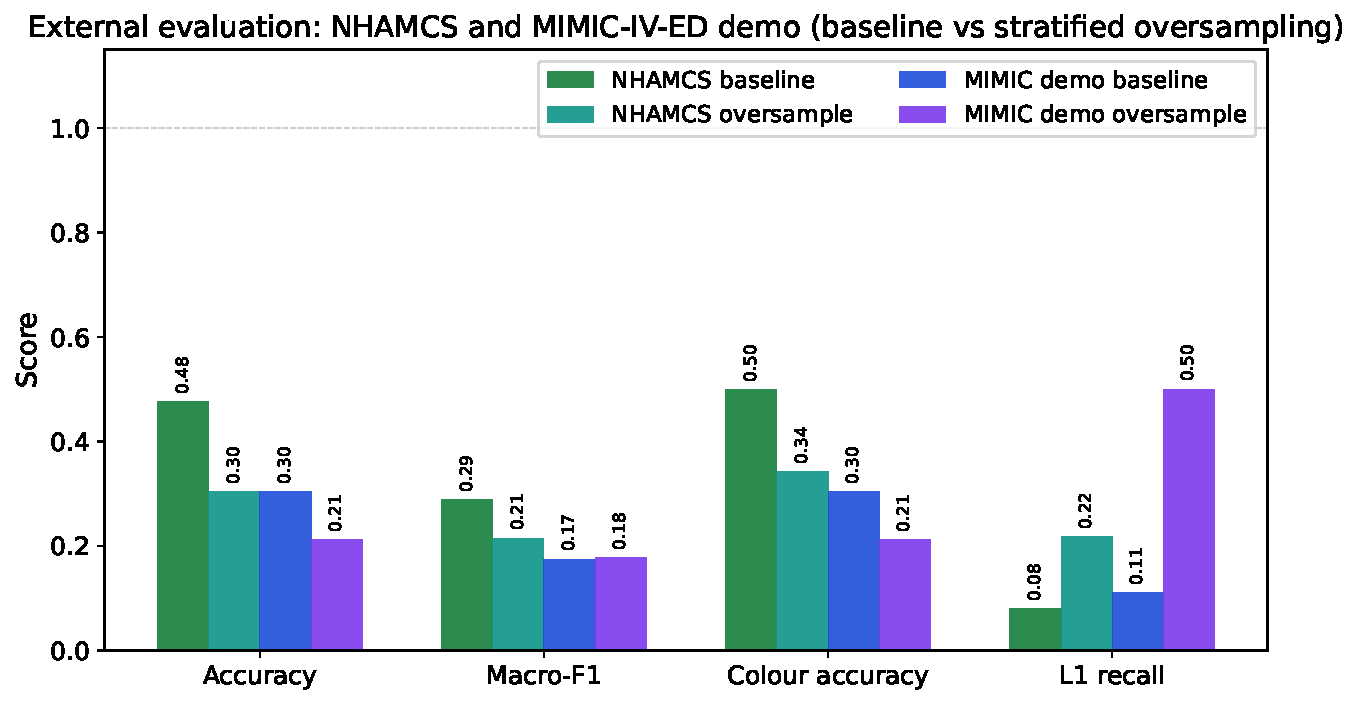
\includegraphics[width=0.92\textwidth]{figures/ch4/external_metrics_compare.pdf}
\caption{External headline metrics on NHAMCS (\(N=12{,}000\) stratified subsample) and MIMIC-IV-ED demo (\(N=207\)): baseline versus stratified oversampling.}
\label{fig:external-metrics-compare}
\end{figure}

Figure~\ref{fig:external-metrics-compare} plots the same accuracy, macro-F1, colour accuracy, and Level~1 recall values as Table~\ref{tab:external-metrics}, so the baseline--oversample contrast is readable before the bootstrap intervals and confusion matrices below.

\begin{figure}[H]
\centering
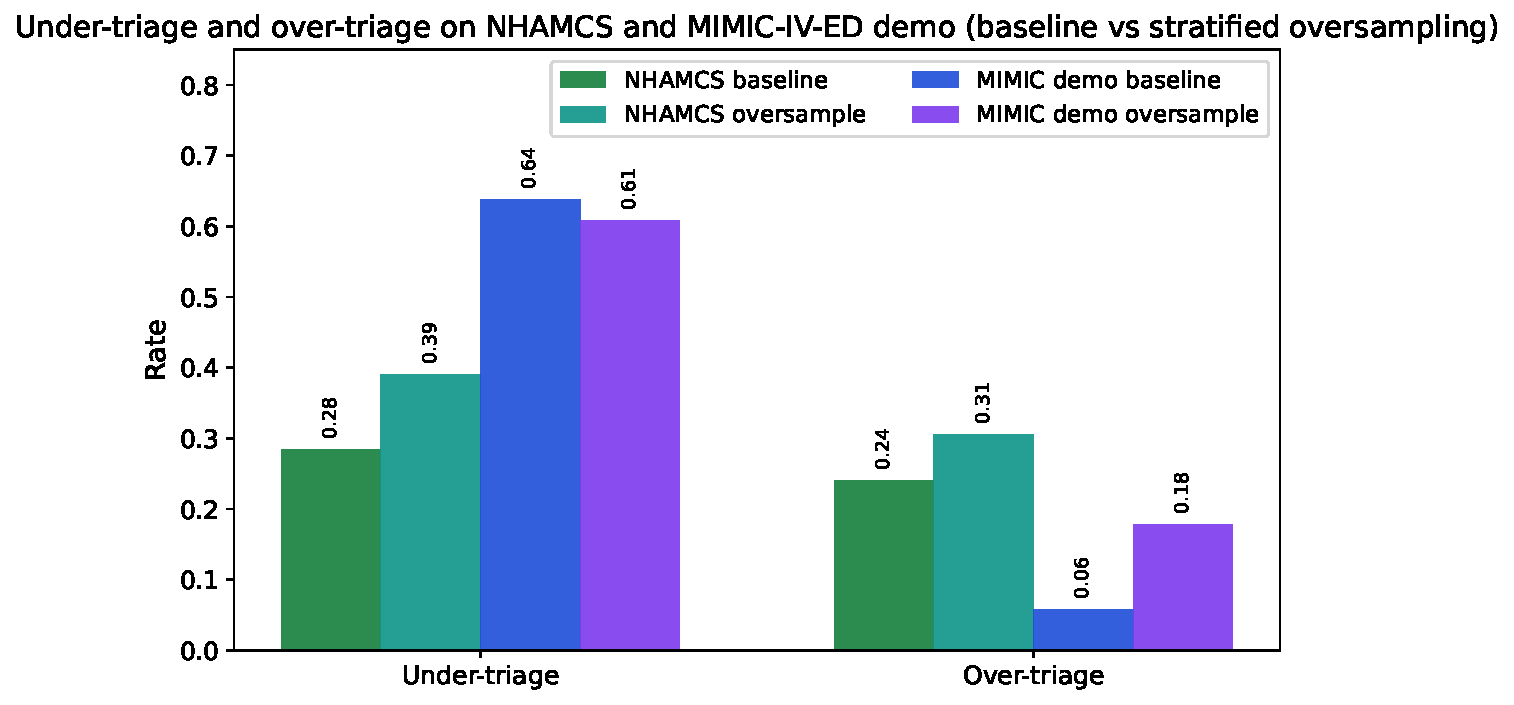
\includegraphics[width=0.92\textwidth]{figures/ch4/external_under_over_triage.pdf}
\caption{Under-triage and over-triage rates on NHAMCS (\(N=12{,}000\) stratified subsample) and MIMIC-IV-ED demo (\(N=207\)): baseline versus stratified oversampling.}
\label{fig:external-under-over-triage}
\end{figure}

Under-triage (predicted less urgent than gold) is the safety failure mode: urgent language is routed too late. Over-triage (predicted more urgent than gold) is false escalation that loads acute streams and staff. Figure~\ref{fig:external-under-over-triage} shows that on NHAMCS, stratified oversampling raises \emph{both} under-triage (28.39\% to 39.03\%) and over-triage (24.01\% to 30.52\%) even while Level~1 recall rises (Figure~\ref{fig:external-metrics-compare}, Table~\ref{tab:external-metrics}), so sensitivity gains are not a free improvement in directional error. On the MIMIC demo, baseline under-triage is already high (63.77\%); oversampling mainly increases over-triage (5.80\% to 17.87\%). These patterns reinforce mandatory nurse override under domain shift \citep{Berkowitz2019}.

\paragraph{Bootstrap uncertainty (what, why, and how to read the intervals).}
The intervals below are derived from the same confusion-matrix cell counts that the figures immediately after expand into readable error patterns. Point estimates in Table~\ref{tab:external-metrics} do not show sampling uncertainty. A \textbf{bootstrap 95\% confidence interval} answers a different question: if we resample this evaluation set many times, in what range does the metric usually fall? It is \emph{not} a claim of clinical certainty at \examplehospital{}.

\textbf{What was computed.} For each published confusion matrix, the cell counts were expanded into \(N\) pairs \((y,\hat{y})\). Then \(B=2000\) ordinary bootstrap resamples (with replacement, seed~42) recomputed five-class accuracy, colour accuracy after \(f_{\mathrm{SATS}}\), and Level~1 (Red) recall. The 2.5th and 97.5th percentiles of those \(B\) values form the percentile 95\% CI in Table~\ref{tab:bootstrap-cis}.

\textbf{Why bootstrap, and why NHAMCS is primary.} Level~1 is scarce (175 true Reds on the NHAMCS subsample; only 18 on the MIMIC demo), so a few additional hits or misses move Red recall substantially. Oversampling also claims a clear accuracy drop and a Red-recall rise; those claims should be checked against sampling noise rather than two-decimal point estimates alone. The \textbf{detailed} reading centres on NHAMCS because it is the main published evaluation set (\(N=12{,}000\)). The MIMIC open demo (\(N=207\)) is a secondary transfer check: the same bootstrap procedure was applied, but with so few Reds the intervals are very wide, so MIMIC CIs document uncertainty on that small set rather than support precise sensitivity claims.

\begin{table}[H]
\centering
\footnotesize
\setlength{\tabcolsep}{3.5pt}
\begin{tabular}{|l|l|c|c|}
\hline
\textbf{Checkpoint} & \textbf{Metric} & \textbf{Estimate} & \textbf{95\% bootstrap CI} \\
\hline
NHAMCS baseline & Five-class Acc & 0.4760 & \([0.4670,\,0.4847]\) \\
NHAMCS baseline & Colour Acc & 0.4995 & \([0.4903,\,0.5082]\) \\
NHAMCS baseline & Recall L1 (Red) & 0.0800 & \([0.0435,\,0.1236]\) \\
\hline
NHAMCS overs. & Five-class Acc & 0.3045 & \([0.2960,\,0.3132]\) \\
NHAMCS overs. & Colour Acc & 0.3423 & \([0.3336,\,0.3513]\) \\
NHAMCS overs. & Recall L1 (Red) & 0.2171 & \([0.1579,\,0.2784]\) \\
\hline
MIMIC demo base. & Five-class Acc & 0.3043 & \([0.2464,\,0.3671]\) \\
MIMIC demo base. & Colour Acc & 0.3043 & \([0.2464,\,0.3671]\) \\
MIMIC demo base. & Recall L1 (Red) & 0.1111 & \([0.0000,\,0.2667]\) \\
\hline
MIMIC demo overs. & Five-class Acc & 0.2126 & \([0.1594,\,0.2705]\) \\
MIMIC demo overs. & Colour Acc & 0.2126 & \([0.1594,\,0.2705]\) \\
MIMIC demo overs. & Recall L1 (Red) & 0.5000 & \([0.2631,\,0.7334]\) \\
\hline
\end{tabular}
\caption{Bootstrap 95\% CIs (\(B=2000\), seed~42) for NHAMCS (\(N=12{,}000\)) and the MIMIC-IV-ED demo (\(N=207\)). Primary interpretation is NHAMCS; MIMIC rows document uncertainty on the small secondary transfer set. Intervals quantify sampling uncertainty on each evaluation set, not clinical certainty at \examplehospital{}.}
\label{tab:bootstrap-cis}
\end{table}

\textbf{Significance on NHAMCS.} Five-class accuracy for the baseline is \(0.476\) with a tight interval \([0.467,\,0.485]\), reflecting the large sample. The oversampled checkpoint falls to \(0.305\) \([0.296,\,0.313]\); the two intervals do not overlap under this resampling scheme, so the accuracy drop is stable, not a fluke of one draw. Colour accuracy follows the same pattern (baseline about \(0.500\) versus oversample about \(0.342\)), and colour accuracy remains slightly above five-class accuracy because Levels~4 and~5 both map to Green under \(f_{\mathrm{SATS}}\). Red recall is the clinically important but noisy quantity: baseline \(0.080\) sits in a wide interval \([0.043,\,0.124]\) because only \(175\) true Level~1 cases are available. Oversampling raises the point estimate to \(0.217\) \([0.158,\,0.278]\). Those Red-recall intervals do not overlap the baseline interval here, which supports a real sensitivity gain for RQ4 / Finding~3, yet the absolute level remains modest (even the upper end stays below about \(0.28\)). The bootstrap therefore strengthens an honest trade-off story: oversampling moves Red recall up and overall accuracy down in a resampling-stable way, while still leaving critical-case detection too weak for unsupervised Red screening.

\textbf{Significance on the MIMIC demo.} On the open demo, baseline five-class (and colour) accuracy is \(0.304\) \([0.246,\,0.367]\); oversampling lowers it to \(0.213\) \([0.159,\,0.271]\). Red recall moves from \(0.111\) \([0.000,\,0.267]\) to \(0.500\) \([0.263,\,0.733]\). Because only \(18\) true Level~1 cases exist, the Red intervals span from near zero to high values: a few flips change the estimate dramatically. MIMIC therefore confirms that the evaluation pipeline runs on real Boston ED phrasing and that oversampling can inflate Red hits on a tiny support, but it does \emph{not} justify precise claims about critical-case sensitivity. That is why the narrative weight stays on NHAMCS, with MIMIC reported for completeness. The confusion matrices next show \emph{where} those errors sit on the five-class grid.

\begin{figure}[H]
\centering
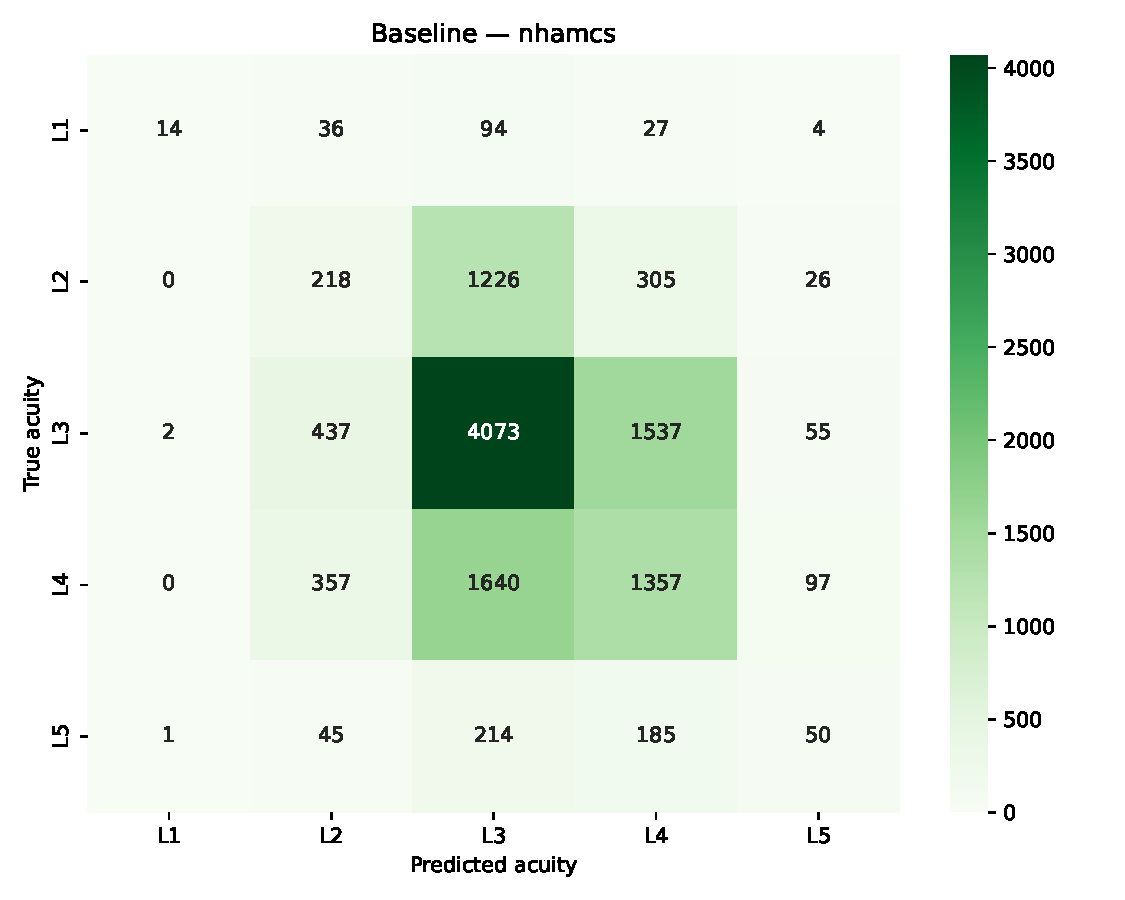
\includegraphics[width=0.82\textwidth]{figures/ch4/nhamcs_baseline_confusion.pdf}
\caption{Baseline BioBERT confusion matrix on NHAMCS stratified subsample (\(N=12{,}000\)). Rows = true acuity; columns = prediction. Dark diagonal cells are correct predictions; off-diagonal mass is triage error.}
\label{fig:confusion-nhamcs-baseline}
\end{figure}

The NHAMCS baseline matrix shows substantial off-diagonal mass. Of 175 true Level~1 cases, only 14 are recovered; 36 are predicted Level~2 (Orange) and 94 Level~3 (Yellow). Under-triage of critical presentations therefore dominates residual error on this US survey set.

\begin{figure}[H]
\centering
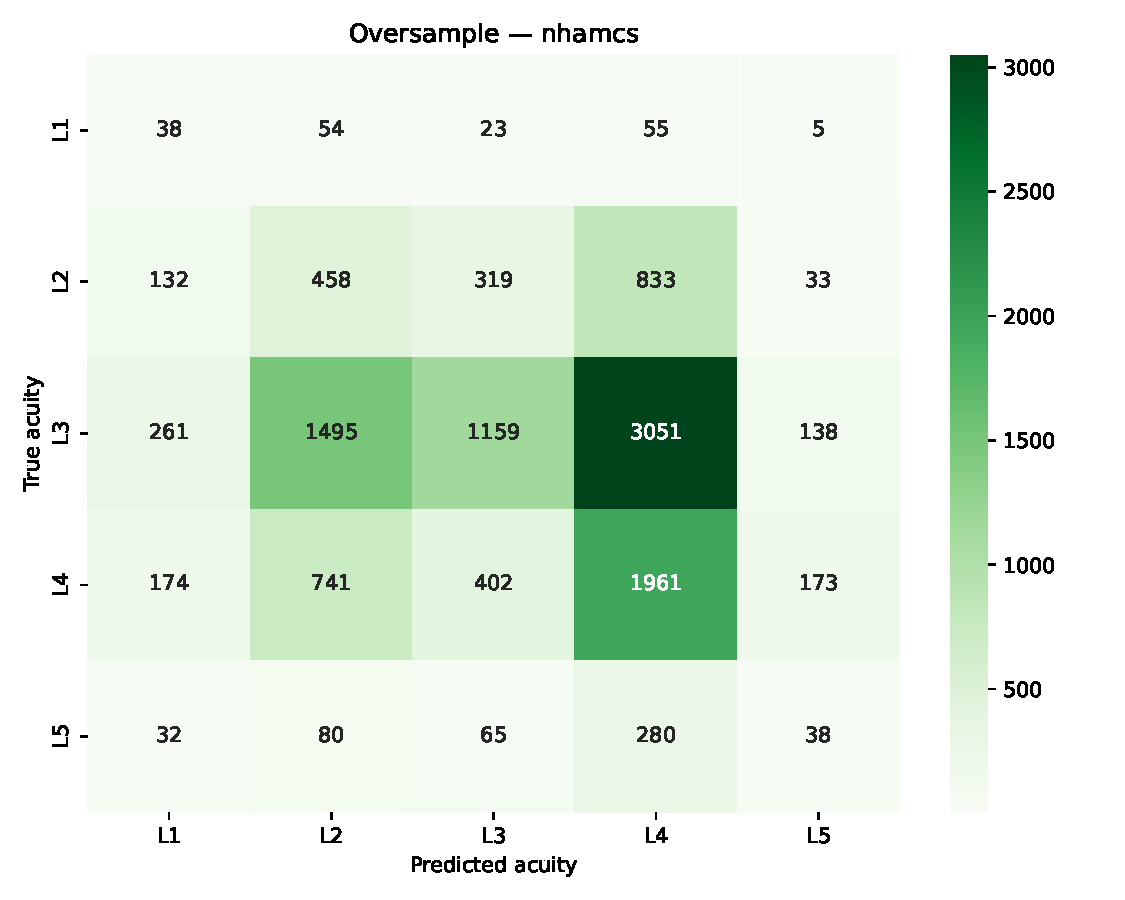
\includegraphics[width=0.82\textwidth]{figures/ch4/nhamcs_oversample_confusion.pdf}
\caption{Stratified-oversampling BioBERT confusion matrix on the same NHAMCS subsample. Dark diagonal cells are correct predictions; off-diagonal mass is triage error.}
\label{fig:confusion-nhamcs-oversample}
\end{figure}

Stratified oversampling raises NHAMCS Level~1 recall from 8.00\% to 21.71\% but lowers overall accuracy to 30.45\% and Level~1 precision to 5.97\%: more false urgent alerts accompany the sensitivity gain. As visually demonstrated by the drop in the Accuracy bars in Figure~\ref{fig:external-metrics-compare}, stratified oversampling trades overall exact-match accuracy to raise Level~1 recall (Table~\ref{tab:external-metrics}). The baseline checkpoint remains the project default unless stakeholders explicitly prioritise Red sensitivity over precision \citep{Berkowitz2019}.

\subsection{MIMIC-IV-ED demo results}
\label{sec:mimic-results}

On the open MIMIC-IV-ED demo (\(N=207\)), baseline accuracy is 30.43\% with colour accuracy 30.43\% and high under-triage (63.77\%). As shown in the baseline matrix (Figure~\ref{fig:confusion-mimic-baseline}), the model correctly recovers only 2 of 18 true Level~1 cases. With stratified oversampling (Figure~\ref{fig:confusion-mimic-oversample}), this increases to 9 of 18 cases (50.00\% recall), though the matrix shows a corresponding spread of false positives across Levels~2 and~3, and overall accuracy falls to 21.26\%. These demo figures validate the evaluation pipeline on real Boston ED phrasing but are not substitutes for a full credentialed MIMIC-IV-ED v2.2 extract \citep{mimicived2023}.

\begin{figure}[H]
\centering
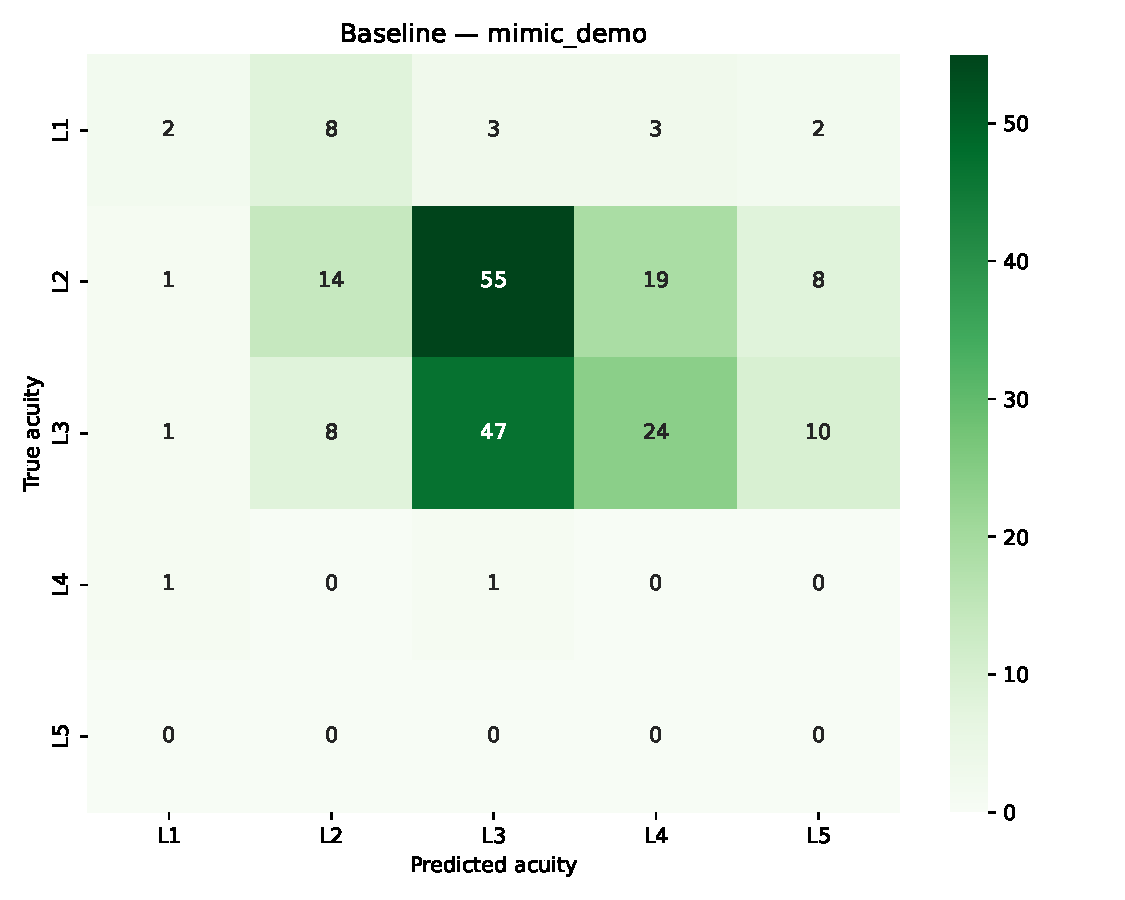
\includegraphics[width=0.82\textwidth]{figures/ch4/mimic_demo_baseline_confusion.pdf}
\caption{Baseline BioBERT confusion matrix on MIMIC-IV-ED demo (\(N=207\)). Rows = true acuity; columns = prediction. Dark diagonal cells are correct predictions; off-diagonal mass is triage error.}
\label{fig:confusion-mimic-baseline}
\end{figure}

\begin{figure}[H]
\centering
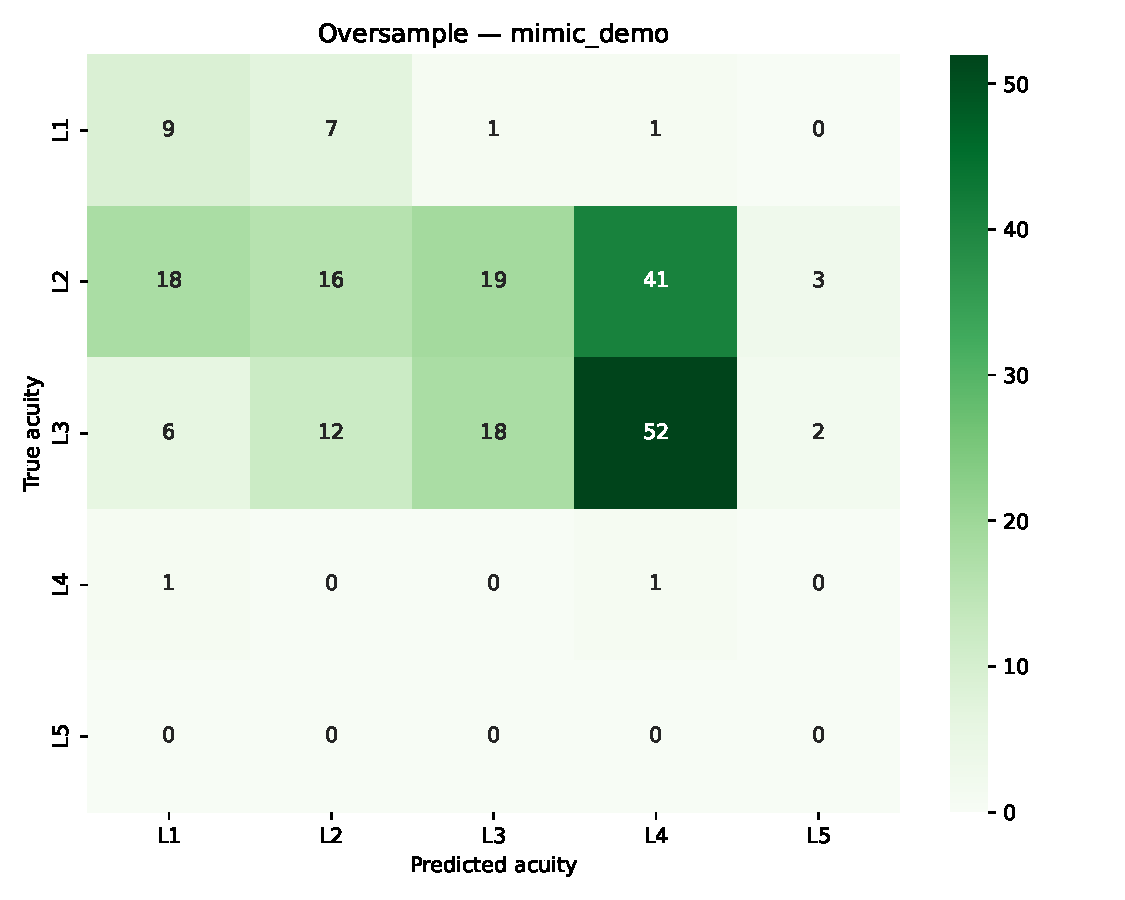
\includegraphics[width=0.82\textwidth]{figures/ch4/mimic_demo_oversample_confusion.pdf}
\caption{Stratified-oversampling BioBERT confusion matrix on MIMIC-IV-ED demo. Dark diagonal cells are correct predictions; off-diagonal mass is triage error.}
\label{fig:confusion-mimic-oversample}
\end{figure}

\subsection{Colour accuracy and under/over-triage}

Mapping levels through \(f_{\mathrm{SATS}}\) (Table~\ref{tab:fsats-esi}) yields 4-colour accuracy at or above five-class accuracy when Levels~4 and~5 both map to Green. On NHAMCS baseline, colour accuracy (49.95\%) slightly exceeds five-class accuracy (47.60\%). Critical under-triage of true Red to non-Red remains high (92.00\% baseline NHAMCS; 78.29\% oversampled), reinforcing mandatory nurse override for urgent language \citep{Berkowitz2019}.

\subsection{Inference latency}
\label{sec:latency}

Real-time intake requires sub-second response \citep{stewart2023nlp}. Latency in Table~\ref{tab:external-metrics} is a property of the BioBERT forward pass at project length \(M=128\) on the evaluation hardware, not a dataset-specific accuracy score. The published timing benchmark is therefore the NHAMCS stratified subsample (\(N=12{,}000\)), which is large enough for stable median and tail estimates: baseline median latency \(\approx 94\)\,ms (p95 \(\approx 124\)\,ms); the stratified-oversampling checkpoint is similar (p50 \(\approx 96\)\,ms). Both respond in well under one second, supporting chatbot intake before nurse vitals are recorded.

MIMIC-IV-ED demo columns in the same table show n/a for latency by design. That demo (\(N=207\)) is used for external accuracy, colour accuracy, and under/over-triage only. A second latency estimate on so few batches would not change the operational sub-second claim and would overstate the precision of a short timing sample. The same checkpoints and the same \(M=128\) truncation are used on both externals, so the NHAMCS p50 already represents chatbot response time at intake.

\begin{remark}
External metrics are substantially lower than earlier Triagegeist in-distribution figures, as expected under geographic and demographic domain shift (Chapter~\ref{ch:conclusion}). Text still carries a partial acuity signal, but the chatbot must remain nurse-overridable.
\end{remark}

\section{Pathway routing at \examplehospital{}}
\label{sec:pathway-results}

The complete five-scenario pathway map (gate reject plus Red, Orange, Yellow, Green) is specified in Tables~\ref{tab:pathway-scenarios} and~\ref{tab:pathway-examples} and illustrated in Figure~\ref{fig:pathway-map}. Each scenario assigns primary clinical departments, support actions across Nursing, Pharmacy, Health Information, Hospital Information Technology, Administration, and Accounts, and an escalation rule \citep{satsmanual,Rominski2014}.

\subsection{Nurse triage vs chatbot response}
\label{sec:nurse-vs-chatbot}

Table~\ref{tab:nurse-vs-chatbot} contrasts manual nurse triage with the hospital chatbot on dimensions relevant to intake at \examplehospital{}. Nurse-side timings are drawn from published LMIC triage literature; chatbot timings are measured on the external evaluation hardware.

\begin{table}[H]
\centering
\small
\begin{tabular}{|p{3.2cm}|p{5.2cm}|p{5.2cm}|}
\hline
\textbf{Dimension} & \textbf{Manual nurse triage} & \textbf{Hospital chatbot (this project)} \\
\hline
Time to first acuity signal &
Queue-dependent; LMIC intake often delayed minutes to hours before nurse contact \citep{kathsats,Mitchell2023,Nurchis2025} &
Approximately 94--100\,ms inference on evaluation hardware (Table~\ref{tab:external-metrics}) \\
Inputs used &
Chief complaint + vitals + TEWS + clinical judgment \citep{satsmanual} &
Text-only chief complaint; TEWS applied separately by nurse (Section~\ref{sec:tews}) \\
Output &
SATS colour + bedside assessment &
SATS colour + pathway card + confidence score \\
Validation basis &
Live clinical decision at triage desk &
External offline agreement on MIMIC/NHAMCS text (Section~\ref{sec:nhamcs-results}) \\
Role at \examplehospital{} &
Authoritative triage &
Triage assist at arrival; nurse override mandatory for low confidence and all vitals \citep{stewart2023nlp} \\
\hline
\end{tabular}
\caption{Manual nurse triage versus chatbot assist at intake.}
\label{tab:nurse-vs-chatbot}
\end{table}

Once the chatbot assigns a colour in approximately 100\,ms, pathway timer rules take effect: Orange cases require clinician contact within ten minutes, Yellow within 60 minutes, and Green within four hours (Section~\ref{sec:pathways}, Table~\ref{tab:pathway-scenarios}) \citep{satsmanual,Sundstrom2014}. The chatbot does not replace nurse assessment; it is intended to provide an immediate acuity signal that could reduce queue time before \emph{any} routing decision relative to waiting for a free triage nurse \citep{Mitchell2023,Nurchis2025}.

\textbf{Gate rejection.} Non-clinical input receives no colour; Nursing re-prompts for a chief complaint. This prevents meaningless acuity scores and keeps acute queues free of idle interactions.

\textbf{Red.} Life-threatening text (e.g.\ crushing chest pain with dyspnoea) routes immediately to Surgery and Internal Medicine with Code Red alerts via HIT. Administration bypasses routine registration so resuscitation is not delayed \citep{satsmanual}.

\textbf{Orange.} Very urgent complaints (e.g.\ severe abdominal pain in pregnancy) activate Internal Medicine, Surgery, or Obstetrics and Gynaecology within ten minutes, with stat Diagnostics and a head-nurse escalation if unclaimed.

\textbf{Yellow.} For the running illustrative complaint (\runningcomplaint{}), the model assigns level 3 at approximately 72\% confidence. The pathway card routes to the Outpatient urgent stream and parallel Diagnostics under the adult ASTS default; Pediatrics applies only under the prototype lexical child-marker rule (Section~\ref{sec:pathways}), which is not a reliable paediatric identifier. Nursing sets a 60-minute reassessment timer.

\textbf{Green.} Under the proposed routing, routine presentations (e.g.\ dental pain without fever) are intended to divert to Outpatient, Dental, Eye, or Public and Preventive Health within four hours, which may support reduced congestion in acute waiting areas \citep{Yilmaz2021,Sundstrom2014}.

Classification output (colour + confidence + department list) is the machine-readable input to this routing layer. External evaluation (Section~\ref{sec:nhamcs-results}) bounds offline reliability under domain shift; live intake at \examplehospital{} still requires nurse override.

\section{Discussion: anticipated impact on healthcare delivery}
\label{sec:impact}

The following discussion interprets how the chatbot \emph{could} support hospital flow at \examplehospital{}, drawing on external metrics where available and on published triage literature elsewhere. These paragraphs are not measured outcome results. No prospective waiting-time trial has yet been conducted at \examplehospital{} \citep{Mitchell2023}.

\subsection{Functional chatbot and workflow improvement}

We anticipate a functional chatbot that suggests ESI-style urgency from a single chief complaint and supports hospital workflow by recommending a SATS-aligned colour and department direction at intake \citep{stewart2023nlp,Mitchell2023}. External NHAMCS evaluation reports 47.60\% five-class accuracy and 49.95\% colour accuracy for the baseline checkpoint (Section~\ref{sec:nhamcs-results}), indicating that text carries a partial acuity signal under domain shift rather than near-perfect agreement. Median inference latency of approximately 94--100\,ms on evaluation hardware supports rapid digital response at arrival (Table~\ref{tab:nurse-vs-chatbot}).

Figure~\ref{fig:anticipated-workflow} compares \emph{time to computational acuity signal}: traditional intake (top) waits for a nurse before any colour exists; chatbot-assisted intake (bottom) produces a model colour recommendation in tens of milliseconds while nurse vitals (TEWS) still run in parallel. The figure does \emph{not} claim that total time from arrival to definitive clinical assessment equals inference latency.

\begin{figure}[H]
\centering
\resizebox{\textwidth}{!}{%
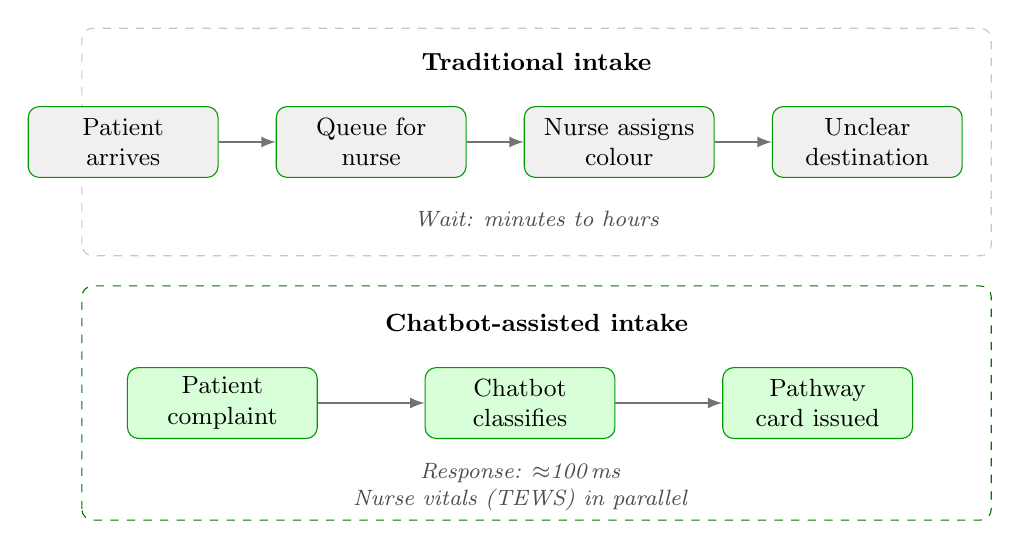
\begin{tikzpicture}[
  x=1.05cm, y=0.85cm,
  title/.style={font=\small\bfseries, anchor=center},
  box/.style={draw=green!60!black, rectangle, fill=green!10, text width=2.2cm, align=center,
    minimum height=0.9cm, rounded corners, font=\small, inner sep=3pt},
  old/.style={box, fill=gray!12},
  new/.style={box, fill=green!15},
  arrow/.style={->, >=latex, thick, draw=black!55},
  foot/.style={font=\footnotesize\itshape, text=black!70, align=center}]
  % Top panel: Traditional
  \node[title] at (5.0, 7.2) {Traditional intake};
  \draw[dashed, rounded corners, draw=gray!45] (-0.5, 4.3) rectangle (10.5, 7.7);
  \node[old] (q) at (0, 6.0) {Patient\\arrives};
  \node[old] (wait) at (3.0, 6.0) {Queue for\\nurse};
  \node[old] (nurse) at (6.0, 6.0) {Nurse assigns\\colour};
  \node[old] (unclear) at (9.0, 6.0) {Unclear\\destination};
  \draw[arrow] (q) -- (wait);
  \draw[arrow] (wait) -- (nurse);
  \draw[arrow] (nurse) -- (unclear);
  \node[foot] at (5.0, 4.85) {Wait: minutes to hours};
  % Bottom panel: Chatbot-assisted
  \node[title] at (5.0, 3.3) {Chatbot-assisted intake};
  \draw[dashed, rounded corners, draw=green!45!black] (-0.5, 0.35) rectangle (10.5, 3.85);
  \node[new] (c) at (1.2, 2.1) {Patient\\complaint};
  \node[new] (bot) at (4.8, 2.1) {Chatbot\\classifies};
  \node[new] (card) at (8.4, 2.1) {Pathway\\card issued};
  \draw[arrow] (c) -- (bot);
  \draw[arrow] (bot) -- (card);
  \node[foot] at (4.8, 1.05) {Response: \(\approx\)100\,ms};
  \node[foot] at (4.8, 0.65) {Nurse vitals (TEWS) in parallel};
\end{tikzpicture}}
\caption{Time to computational acuity signal at \examplehospital{} (schematic). \textbf{Top:} traditional intake may wait minutes to hours before a nurse assigns colour. \textbf{Bottom:} chatbot issues an ESI-style / \(f_{\mathrm{SATS}}\) colour recommendation in \(\approx\)100\,ms inference time; nurse TEWS vitals continue in parallel. This is \emph{not} a measured reduction in total door-to-provider waiting time. Colour routing (Red/Orange vs Green) is detailed in Section~\ref{sec:pathway-results}.}
\label{fig:anticipated-workflow}
\end{figure}

The stacked workflow diagram has two panels read left to right. The top panel is traditional intake (arrive \(\rightarrow\) queue \(\rightarrow\) nurse assigns colour \(\rightarrow\) unclear destination); the bottom panel is chatbot-assisted intake (complaint \(\rightarrow\) chatbot classifies \(\rightarrow\) pathway card issued). Pathway design comes from Chapter~\ref{ch:method}, chatbot latency from the external evaluation in Section~\ref{sec:latency}, and traditional wait times from LMIC triage literature \citep{kathsats,Mitchell2023}. The top footnote reads ``Wait: minutes to hours''; the bottom footnotes read ``Response: \(\approx\)100\,ms'' and ``Nurse vitals (TEWS) in parallel''. Red/Orange fast-track and Green digital queue are developed in Section~\ref{sec:pathway-results}. The figure therefore contrasts slow nurse-queue intake with immediate chatbot classification while making clear that nurse assessment is not replaced \citep{satsmanual,stewart2023nlp}.

\subsection{Anticipated initial triage wait times}

These paragraphs remain hypothetical. Published triage literature suggests that wait times for \emph{initial} triage assessment \emph{could} fall if patients interact with a bot immediately rather than queue solely for a nurse \citep{Mitchell2023,Nurchis2025}, but no door-to-provider trial was run here. External evaluation only shows that the model can assign a colour and pathway recommendation in approximately 100\,ms once valid clinical text is submitted (Table~\ref{tab:nurse-vs-chatbot}). Protocol design \emph{intends} Green cases to be digitally queued and Red/Orange cases to be fast-tracked (Table~\ref{tab:pathway-scenarios}); whether that shortens overall waiting duration at \examplehospital{} is unmeasured \citep{Sundstrom2014,Yilmaz2021}.

\subsection{Critical-case sensitivity and safety implications}

The principal limitation of the baseline system is poor recall for the most urgent class under external domain shift. On NHAMCS, baseline Level~1 (Red) recall is only 8.00\% (support 175): about 92\% of true Red cases were not identified as Red, with most missed cases predicted as Orange or Yellow (Figure~\ref{fig:confusion-nhamcs-baseline}). Stratified oversampling raises Level~1 recall to 21.71\% at large cost to precision, so no satisfactory operating point has yet been established for unsupervised critical-case screening. High offline sensitivity for critical cases is therefore \emph{not} demonstrated on US external text; nurse override and prospective audit remain essential \citep{Berkowitz2019}. Waiting-time deterioration increases adverse outcomes when triage colour is not reassessed \citep{Nurchis2025}; digital timers on Orange and Yellow pathway cards are \emph{intended} to reduce this risk, not proven to do so in this project \citep{satsmanual}.

\subsection{Patient satisfaction and appropriate categorisation}

Patient satisfaction and live clinical confirmation rates were not measured. A prospective pilot \emph{could} ask whether quick pathway feedback improves perceived guidance \citep{stewart2023nlp}; offline NHAMCS/MIMIC agreement alone cannot answer that (Section~\ref{sec:nhamcs-results}).

\subsection{Staff workload and public-health insights}

Staff workload reduction and public-health surveillance benefits are likewise unmeasured hypotheses. Nursing documentation burden \emph{might} shift if intake text capture is partly automated \citep{stewart2023nlp,Mitchell2023}; the gate can reject non-clinical chat before BioBERT (Section~\ref{sec:gate}). Any future aggregation of anonymised complaints for trend analysis would require privacy and governance review first.

\subsection{Success criteria}

Prospective success at \examplehospital{} would be judged by measured flow, nurse override rates, and adverse events or delays attributable to triage, not by offline Acc alone \citep{Rominski2014,kathsats}. Those criteria are targets for future evaluation, not results claimed in this thesis.
\textbf{Limitations.} External metrics measure classification accuracy on US chief-complaint text, not patient outcomes, waiting-time reduction, or satisfaction scores at \examplehospital{} \citep{Mitchell2023,Nurchis2025}. Prospective local validation is required. Training-data class imbalance and NHAMCS Level~1 scarcity widen uncertainty on rare urgent classes; deployment should treat low-confidence or contradictory presentations as mandatory nurse review \citep{Berkowitz2019,satsmanual}. Stratified oversampling increases Red recall on NHAMCS but sharply lowers Red precision; the baseline checkpoint is the project default unless clinical stakeholders prioritise sensitivity over precision.

\section{Discussion of findings}
\label{sec:discussion}

Combining the model architecture analysis with the external metrics suggests five findings, addressing the research questions in Chapter~\ref{ch:intro}.

\textbf{Finding 1.} BioBERT learns a partial acuity signal from free text after Stage~3 fine-tuning. Naive bounds remain near chance without that supervised step.

\textbf{Finding 2.} External domain shift substantially degrades performance relative to retired in-distribution Triagegeist headlines; NHAMCS baseline accuracy is 47.60\% with ordinal MAE \(0.627\).

\textbf{Finding 3.} Class rebalancing (stratified oversampling) increases Red recall (8.00\%\(\to\)21.71\% on NHAMCS) but introduces many false urgent predictions and worsens MAE, so no free lunch exists under \(R(\theta)\).

\textbf{Finding 4.} The ESI\(\to\)SATS map \(f_{\mathrm{SATS}}\) is operational rather than clinically validated; colour accuracy is not interchangeable with five-class accuracy because Levels~4 and~5 share Green.

\textbf{Finding 5.} Latency near 94\,ms is suitable for real-time interaction, but latency alone does not establish clinical utility or waiting-time reduction.

\paragraph{Safety posture.}
External five-class accuracy under domain shift does not license unsupervised discharge decisions. The deployed posture is triage assist with nurse override, TEWS in parallel, gate rejection of non-clinical text, and mandatory review when
\[
  \max_c\hat{y}_c < \tau_c
  \quad\text{or}\quad
  \hat{y}_{(1)}-\hat{y}_{(2)} < \delta
\]
(with prototype \(\tau_c=0.60\), \(\delta=0.10\); Section~\ref{sec:e2e}), or when text conflicts with vitals \citep{stewart2023nlp,Berkowitz2019}. That posture is consistent with SATS training manuals and with under-triage quality literature.
